\chapter{Basic Concepts in  Asynchronous Editing}
\label{chap:concepts}

The purpose of this chapter is to briefly introduce several basic concepts which are
strongly related to the field of asynchronous editing. All these concepts will be widely
used throughout the remaining chapters and, therefore, need to be properly (and, if
appropriate) rigorously defined before being actually used. The goal is to sufficiently
accustom the reader with notions like commit, update or check out (as well as many others)
in order for him/her to have the necessary basis to understand the rest of this paper.

\section{Version}

The most basic concept which one comes across when dealing with asynchronous text
editing is known as the \emph{version} of a document. A version represents
the state of the document at a very precise moment in time. Generally, the version
of the document changes every time a user ``tells'' the system that (s)he has brought
one or more changes to the document and desires to make the system (and, through the
system, the other users) aware of his/her changes. Each version of the document is
given a number and a timestamp, both of which uniquely identify it. Version numbers
are generated in increasing order. The \emph{current version} of the document refers
to the version with the greatest number from the set of all available versions.

As a side note, various existing version control systems (see \ref{sec:vcs}) also
introduce more advanced concepts, such as those of \emph{subversion} or \emph{revision}
in addition to that of version. Since such concepts are not used anywhere in this
paper they will be silently ignored.

\section{Version control systems}
\label{sec:vcs}

In \cite{shen02} \emph{version control systems} are introduced as ``widely used
asynchronous collaborative systems in team-working environment, where document
merging is a key function.'' Essentially, the purpose of a version control system
is to provide its users with a history of document versions which dates back to
the beginning of the editing of a document, allow them to retrieve any of these
versions, modify them (ideally, in a concurrent manner) and commit their changes
so that others can become aware of them as well. As mentioned before, versions are usually
identified by their date or by a version number. Generally, the system should allow
the retrieval of any of the two identifiers provided that the other one is known.

For the particular case of software development, a version control system allows
programmers involved in the project to keep track of all the changes they have made
to their files during the development process. This is especially useful when, after
several changes, certain functionalities ceased to behave as expected
or certain bugs seemed to have appeared. In such cases, a version control system
acts as an supplemental insurance that the already achieved goals will never be
lost.

A rather interesting description of \emph{version control} itself can be found
in \cite{collins04} and reads:
\begin{quote}
Version control is the art of managing changes to information. It has long been a critical
tool for programmers, who typically spend their time making small changes to software and
then undoing those changes the next day. But the usefulness of version control software extends
far beyond the bounds of the software development world. Anywhere you can find people using
computers to manage information that changes often, there is room for version control.
\end{quote}

The basic configuration of a version control system can be illustrated by Figure \ref{fig:vcs}.
As shown, the main actors in a version control system are the \emph{repository} and the
\emph{client}s, the functions of which will be detailed in the subsequent sections. Essentially,
the repository is a container of all versions of the document, while the clients connect
to the repository through a network (may it be a LAN, the Internet or any other type of network)
in order for them to retrieve and submit document changes (and thus work together as a group).
Clients hold local reflections of some version of the document from the repository (also
known as \emph{working copies}) on which they make all their modifications.

\begin{figure}[ht]
\begin{center}
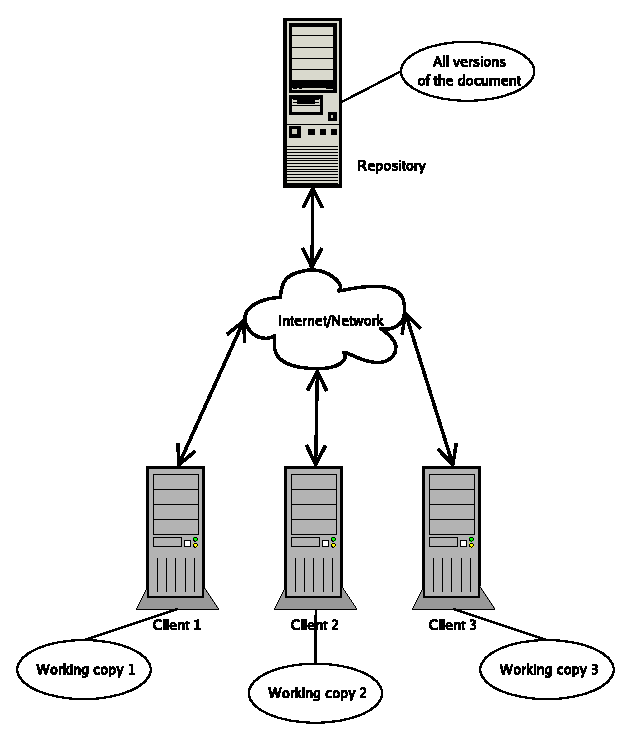
\includegraphics{img/vcs.eps}
\end{center}
\caption{Configuration of a basic version control system}
\label{fig:vcs}
\end{figure}

\section{Repository}

A rough definition of a \emph{repository} could be:

\begin{defi}
A \emph{repository} is a store of items that typically are fetched in order to perform some task.
Items in a repository (such as a document) would be retrieved in order to be used in their own
right. In contrast, data in a database might be used to compute statistics, or to verify access,
or retrieve information associated with a triggering event, rather than used as an artifact
in their own right.
\end{defi}

Particularizing this definition, we could refer to a version control system repository as the
component of the version control systems which holds all the versioned data. It is, in essence, a
\emph{sort of} file server which, in addition to basic file server functions, also memorizes
all the intermediate versions of the files it handles. A repository should provide at least
the two following services for its clients:

\begin{itemize}
\item retrieval of any version of any of the files it stores
\item submission of changes to any of the files it stores from any of its clients and record
      these changes as a new version of the document
\end{itemize}

Apart from these two basic functions, a repository can additionally offer a number of optional
ones, such as:

\begin{itemize}
\item retrieval of the version number of a document based on the date at which it was created
\item retrieval of the date at which a certain version of a document was created
\item support for directories (in addition to files)
\item storage of the name of the person who has brought certain changes to a file
\item etc.
\end{itemize}

\section{Repository client}

The \emph{repository client}s are the actual users which connect to the repository and make
use of the functions it provides. Technically, any number of clients can connect to the
repository and then read or write the stored documents. A client has to read data
from the repository in order to find out about the changes performed by other
clients on the document (this operation is referred to as an  ``update'')
and write data to the repository in order to ``publish'' their own changes (known
as the ``commit'' operation).

\section{Versioning models}

Note: the ideas presented in this section are a slightly modified form of those described in
\cite{collins04}.
\\
\\
Virtually all version control systems are faced with the same fundamental question: how
can they allow all users to access the same document and still ensure that
the changes made by all users are preserved. In other words, how can one make
sure that the changes one user makes will not disappear in the moment another user
\emph{simultaneously} makes other changes? Such cases frequently appear when two
or more users work on the same document at the same time.

If no special care is taken we could be faced with a situation as the following: two
users work concurrently on the same document, each of them making his/her own changes.
One of the users will obviously send his/her changes to the repository first. Later,
the other user will commit (different modifications, naturally) as well. At this point
the changes performed by the first user will not be included in the current version since
the second user was not aware of them (meaning that the copy of the document he had
been working on did not contain the changes made by the first user). The first user's
changes would appear in the history of the document (should one be interested enough
to look for them), but still, they would be missing from the latest version. This is
obviously not the desired behavior of such a system.

\subsection{The Lock-Modify-Unlock Solution}

The most immediate solution to the shared document problem discussed above that comes to
mind is to simply not allow more than one user to make modifications to a document at
any given time. This can be easily achieved by employing a locking policy. This would
essentially mean that when a user wants to edit a document (s)he is only allowed to do
so if the document is not currently locked. If the document is not locked, this user
will lock it (and thus make it impossible for any other user to gain access to it until
it is unlocked by the same user who locked it in the first place) and then be able
to modify to it. Once (s)he has finished working with the document, (s)he will
unlock it so that other users can access it as well. If the document is locked at the
time some user wants to access it, the user will simply have to wait until the user
currently editing the document decides to unlock it.

The \emph{Lock-Modify-Unlock} policy certainly has several severe drawbacks, easily noticeable
even to someone only slightly accustomed to systems based on this policy. Here is a short
list enumerating just some of them:

\begin{itemize}
\item only one user can work on a document at a given moment in time. This is a serious
      limitation, especially for cases when users want to work on totally different parts
      of the document, so they would actually not interfere in any way.
\item the user holding the lock could simply forget to release it once he is finished
      doing his/her modifications, thus blocking all other users from accessing the document.
      This could lead to serious delays for groups working together. Also, network failures
      could also lead to the impossibility of a user releasing the lock with the same
      undesirable consequences.
\item there is no way to allow access to documents based on priorities if the user who has
      locked the document goes offline. Suppose the group policy states that the group leader
      should have priority access to the documents on which the group works, but a certain
      member of the group has locked on ore more of the documents and then went offline. There
      is no way in which the system can forcibly take the lock away (supposedly using a
      mechanism similar to preemption) from the user holding it and give it to the group
      leader.
\end{itemize}

In light of such limitations, it is clear that a new model had to be employed.

\subsection{The Copy-Modify-Merge Solution}
\label{sec:cmm}

Most modern version control systems are built to work in the manner of \emph{Copy-Modify-Merge}
as an alternative to locking: each user checks out a separate working copy from the repository
by making a local image of the original and does all his/her modifications on this copy. This
is done independently of all other users which might be working on their own working copies
of the same original version. When editing is finished, two situations can arise. If only
one user has worked on the document, then his version is simply stored on the repository as
the new version. If, however, two or more users worked concurrently on the document, their
modifications are merged together (either completely automatically or partially automatically
and partially by hand) into a new version (actually, a different version is created on the
repository for each user, but each successive version integrates the modifications introduced
by all versions previous to it regardless of whether they were made concurrently or not).

As mentioned in \cite{ignat04b}, the \emph{Copy-Modify-Merge} technique consists basically
of three operations applied on a shared repository storing multiversioned objects: checkout,
commit and update. These three fundamental operations can be defined as follows:

\begin{defi}
A \emph{checkout} operation is the operation by which a client creates a local working copy
of a user-specified version of an object (more specifically, a document) from the repository.
\end{defi}

\begin{defi}
\label{def:commit}
A \emph{commit} operation is the operation by which the user submits a modified version of
his/her working copy of an object from the repository back to the repository, with the intention
of making it the current version. The commit operation is successful only if the repository
does not contain a more recent version of the object than the one the original working copy
of the client trying to do the commit was a replica of.
\end{defi}

\begin{defi}
An \emph{update} operation performs the merging of the local working copy of the object with
the latest version of that object stored in the repository.
\end{defi}

The most essential, and at the same time difficult, function of asynchronous collaborative systems,
the one which actually differentiates one version control system from another, is the
\emph{merging} done during the update phase. This is the process of integrating two documents
(which are usually modified versions of the same original document) in order to generate a
new document that contains as many of the changes that appear in both documents as possible.

\begin{flushleft}
\begin{figure}[ht]
\begin{flushright}
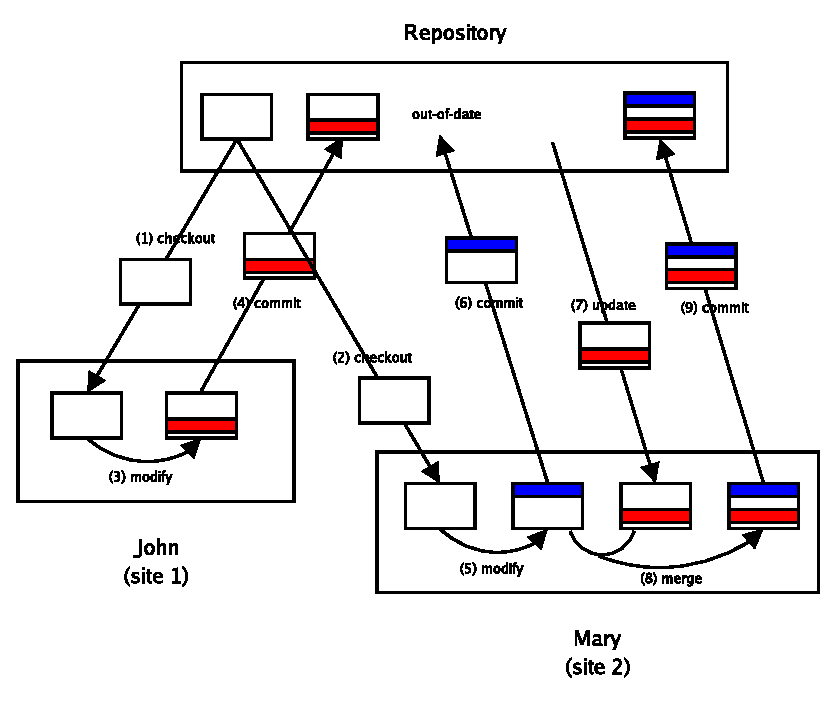
\includegraphics{img/cmm.eps}
\end{flushright}
\caption{A Copy-Modify-Merge scenario}
\label{fig:cmm}
\end{figure}
\end{flushleft}

In order to clarify the inner workings of the \emph{Copy-Modify-Merge} mechanism, we illustrate
a typical usage scenario in Figure \ref{fig:cmm}. In this example, John (the user at site 1) and
Mary (the user at site 2) both checkout the same original version of a document from the repository
roughly at the same time, thus creating two, initially identical, working copies, each in his/her own
private workspace. These are denoted as steps (1) and (2) in the figure. Next, John does his
modifications on his working copy (operation (3) in the figure) and obtains a modified
version of his working copy. When he considers that his work is finished, he goes on to performing
operation (4), namely commit his modified version of the document to the repository. As the
current version on the repository is the same one as the one John's original working copy was
replicating, the commit step ends successfully (see Definition \ref{def:commit}) and the current
version on the repository changes to John's local working copy. In parallel with John,
Mary does her own modifications to her working copy, obviously oblivious of the ones John has
made (step (5) in the figure). After finishing her work she tries to commit her own changes
back to the repository (operation (6)). Her attempt to commit is unsuccessful because, as
the repository puts it, her version is out-of-date. This translates to the fact that the
version she modified is no longer the latest version on the repository. Therefore, as
Definition \ref{def:commit} stipulates, her commit is bound to be unsuccessful. In order to
overcome this problem and actually be able to commit her changes, Mary will first have to do an
update (step (7) in the figure). By doing so, she becomes aware of the modifications John has
made (and successfully committed) and merges (operation (8)) them into her own local working
copy (actually, merges her working copy with the latest version of the document on the repository
and obtains a new document which becomes her current working copy). Thereafter, she retries to
commit her changes (illustrated as step (9)) and, as the working copy she is now considered (by
the repository) to have started working from is a replica of the latest version of the
document on the repository, she succeeds. As one can see, the current version of the document
on the repository after both John and Mary have successfully committed contains both of their
modifications, which is what we wanted in the first place.

As mentioned before as well, the essential operation in this model is the \emph{merging}
operation. Two distinct ways of doing a merge between two documents (usually versions of
the same original document) are effectively employed in production and research
systems today: state-based merging and operation-based merging.

\emph{State-based merging} is a way of merging two documents that only uses information
about the states of the documents, without requiring any information whatsoever about how
one state evolved into another. When a user edits some version of a document, all that he
will have in the end will be the final version (or state) of the document, without the list
of changes that have transformed the initial state into the current one. In order to merge
the two states of the document (in the case of an update, for instance) a comparison
algorithm (such as diff, for example) is used to compute a delta which encapsulates the difference
between the two states. This delta is then applied on one of the document's states
in order to generate the document state that represents the result of the merging. 

\emph{Operation-based merging}, on the other hand, works in a completely different manner.
It essentially stores the information about the evolution of one state of the document into another.
This information is kept under the form of the list of operations that have been performed
in order to transform the initial version of the document into the current one. Merging,
in this case, is done by applying an algorithm that computes the form in which the set
of operations associated with one version of the document have to be applied on the second
version of the document in order to achieve the same effect as if their original form
had been applied on the original version of the document (the original version from which
both versions we are now trying to merge emerged). Once this form is obtained, the operations
(in their modified form) are simply applied on the second document in order to generate
the version representing the result of the merging.

Merging happens at two stages throughout the model, at the committing stage and at the update
stage (\cite{shen02}). Merging at the committing stage takes place when a user wants to
commit his changes and the repository must modify the latest version of the document so
that it reflects the modifications made by the user currently committing. This kind of merge
is actually a very trivial, particular case of the general merge in which all that we have
to do is reapply the operations executed locally by the user on the document version on the
repository (if dealing with operation-based merging) or simply add the new state of the
document (as committed by the user) as the latest version (if dealing with state-based
merging). Merging at the update stage takes place when a commit is unsuccessful due to the
out-of-date problem. Therefore, the user trying to commit has to do an update first in order
to be then able to recommit. As part of this update operation, the user has to merge the
version received from the repository with his/her own working copy. This kind of merging
(at the update stage) is no longer trivial since the two documents that have to be merged
both brought some modifications to a common original version and both sets of modifications
have to appear in the final version. The way to do this has been intuitively described
above (both in the state-based and in the operation-based approach). A more detailed explanation
of how this is actually done in the case of operation-based merging is in fact the subject
of a large part of this paper.